\section{Sample size and power}

%%%%%%%%%%%%%%%%%%%%%%%%%%%%%%%%%%%%

\subsection{Finding a sample size for a certain margin of error}

%%%%%%%%%%%%%%%%%%%%%%%%%%%%%%%%%%%%

\begin{frame}

\dq{A group of researchers wants to test the possible effect of an epilepsy medication taken by pregnant mothers on the cognitive development of their children. As evidence, they want to estimate the IQ scores of three-year-old children born to mothers who were on this particular medication during pregnancy. Previous studies suggest that the standard deviation of IQ scores of three-year-old children is 18 points. How many such children should the researchers sample in order to obtain a 96\% confidence interval with a margin of error less than or equal to 4 points?}

\pause

We know that the critical value associated with the 96\% confidence level: $z^\star = 2.05$. 

\pause

\[ 4 \ge 2.05 * 18 / \sqrt{n} \rightarrow n \ge (2.05 * 18 / 4)^2 = 85.1 \]

\pause

The minimum number of children required to attain the desired margin of error is 85.1. Since we can't sample 0.1 of a child, we must sample at least 86 children (round up, since rounding down to 85 would yield a slightly larger margin of error than desired).

\end{frame}

%%%%%%%%%%%%%%%%%%%%%%%%%%%%%%%%%%%%

\subsection{Power and the Type 2 Error rate}

%%%%%%%%%%%%%%%%%%%%%%%%%%%%%%%%%%%%

\begin{frame}
\frametitle{}

\begin{center}
\begin{tabular}{l l | c c}
\multicolumn{2}{c}{} & \multicolumn{2}{c}{\textbf{Decision}} \\
& & fail to reject $H_0$ &  reject $H_0$ \\
  \cline{2-4}
& $H_0$ true & \onslide<4->{\green{$1 - \alpha$}} & \onslide<2->{\red{Type 1 Error, $\alpha$}} \\
\raisebox{1.5ex}{\textbf{Truth}} & $H_A$ true &  \onslide<3->{\red{Type 2 Error, $\beta$}} & \onslide<5->{\green{Power, $1 - \beta$}} \\
  \cline{2-4}
\end{tabular}
\end{center}

\pause

\begin{itemize}
\item Type 1 error is rejecting $H_0$ when you shouldn't have, and the probability of doing so is $\alpha$ (significance level)

\pause 

\item Type 2 error is failing to reject $H_0$ when you should have, and the probability of doing so is $\beta$ (a little more complicated to calculate)

\pause 

\item \hl{Power} of a test is the probability of correctly rejecting $H_0$, and the probability of doing so is $1 - \beta$

\pause 

\item In hypothesis testing, we want to keep $\alpha$ and $\beta$ low, but there are inherent trade-offs.

\end{itemize}

\end{frame}

%%%%%%%%%%%%%%%%%%%%%%%%%%%%%%%%%%%%

\begin{frame}
\frametitle{Type 2 error rate}

If the alternative hypothesis is actually true, what is the chance that we make a Type 2 Error, i.e. we fail to reject the null hypothesis even when we should reject it?

\begin{itemize}

\item The answer is not obvious.

\item If the true population average is very close to the null hypothesis value, it will be difficult to detect a difference (and reject $H_0$).

\item If the true population average is very different from the null hypothesis value, it will be easier to detect a difference.

\item Clearly, $\beta$ depends on the \hl{effect size} ($\delta$)
\end{itemize}

\end{frame}

%%%%%%%%%%%%%%%%%%%%%%%%%%%%%%%%%%%%

\begin{frame}
\frametitle{Example - Blood Pressure}
{\footnotesize
Blood pressure oscillates with the beating of the heart, and the systolic pressure is defined as the peak pressure when a person is at rest. The average systolic blood pressure for people in the U.S. is about 130 mmHg with a standard deviation of about 25 mmHg. \\
~\\
We are interested in finding out if the average blood pressure of employees at a certain company is \emph{greater} than the national average, so we collect a random sample of 100 employees and measure their systolic blood pressure. What are the hypotheses?

\soln{\only<2->{
\begin{align*}
H_0&: \mu = 130 \\
H_A&: \mu > 130  
\end{align*}
}}

\only<3->{
We'll start with a very specific question -- ``What is the power of this hypothesis test to correctly detect an \emph{increase} of 2 mmHg in average blood pressure?''
}
}
\end{frame}


%%%%%%%%%%%%%%%%%%%%%%%%%%%%%%%%%%%%

\begin{frame}
\frametitle{Calculating power}

The preceding question can be rephrased as ``How likely is it that this test will reject $H_0$ when the true average systolic blood pressure for employees at this company is 132 mmHg?"

~\\
\pause
Hint: Break this down intro two simpler problems
\pause
\begin{enumerate}
\item Problem 1: Which values of $\bar{x}$ represent sufficient evidence to reject $H_0$?
\pause
\item Problem 2: What is the probability that we would reject $H_0$ if $\bar{x}$ had come from $N\left(mean = 132, SE = \frac{25}{\sqrt{100}} = 2.5\right)$, i.e. what is the probability that we can obtain such an $\bar{x}$ from this distribution?
\end{enumerate}
\vspace{-2mm}
~\\
\pause
Determine how power changes as sample size, standard deviation of the sample, $\alpha$, and effect size increases.


\end{frame}


%%%%%%%%%%%%%%%%%%%%%%%%%%%%%%%%%%%%

\begin{frame}
\frametitle{Problem 1}

Which values of $\bar{x}$ represent sufficient evidence to reject $H_0$? \\
(Remember $H_0: \mu = 130$, $H_A: \mu > 130$)

\soln{
\pause
\twocol{0.35}{0.65}
{
{\small
\only<2->{
\[P(Z > z) < 0.05 ~~\Rightarrow~~ z > 1.65 \]
\[\frac{\bar{x}-\mu}{s/\sqrt{n}} > 1.65 \]
\begin{align*}
\bar{x} &> 130 + 1.65 \times 2.5 \\
\bar{x} &> 134.125
\end{align*}
}
}
}
{\vspace{0mm}
\only<2->{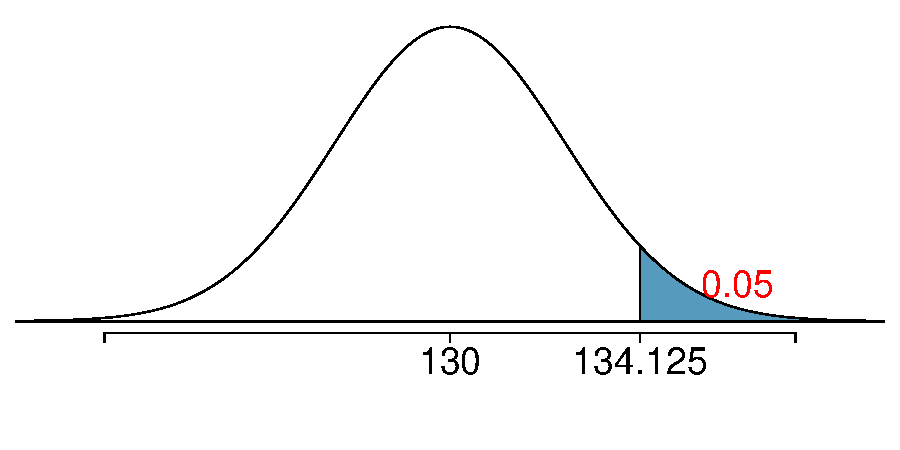
\includegraphics[width=\textwidth]{4-6_samp_size_power/figures/power/powerProblem1}}
}
\only<3->{
Any \red{$\bar{x} > 134.125$} would be sufficient to reject $H_0$ at the 5\% significance level.
}
}
\end{frame}

%%%%%%%%%%%%%%%%%%%%%%%%%%%%%%%%%%%%

\begin{frame}
\frametitle{Problem 2}
{\footnotesize
What is the probability that we would reject $H_0$ if $\bar{x}$ did come from $N(mean = 132, SE = 2.5)$.

\soln{
~\\
\pause
{\small This is the same as finding the area above $\bar{x} = 134.125$ if $\bar{x}$ came from $N(132, 2.5)$.}
\pause
\soln{{\small
\twocol{0.4}{0.6}
{
{\small
\begin{align*}
Z &= \frac{134.125 - 132}{2.5} \\
&= 0.85 \\
\\
P(Z > 0.85) &= 1 - 0.8023 \\
&= 0.1977
\end{align*}
}
}
{\vspace{0mm}
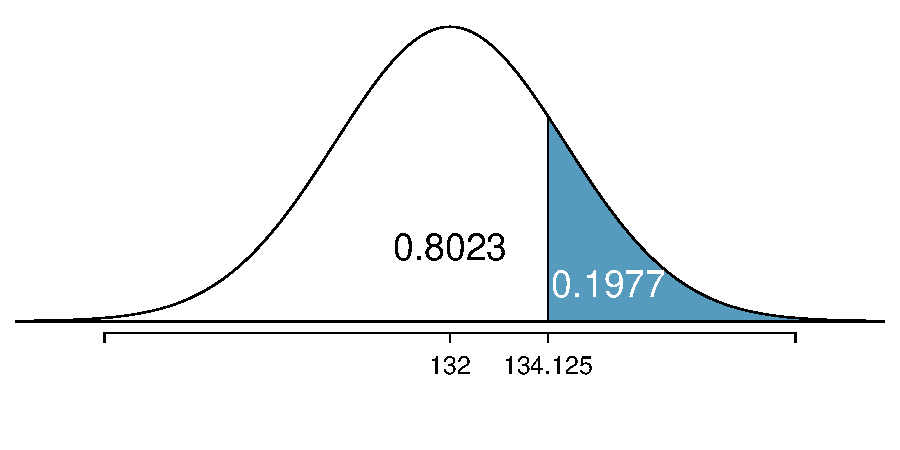
\includegraphics[width=\textwidth]{4-6_samp_size_power/figures/power/powerProblem2}
}
}
\pause
The probability of rejecting $H_0: \mu = 130$, if the true average systolic blood pressure of employees at this company is 132 mmHg, is 0.1977 which is the power of this test.\\
Therefore, $\beta = 0.8023$ for this test.}
}
}
\end{frame}

%%%%%%%%%%%%%%%%%%%%%%%%%%%%%%%%%%%%

\begin{frame}
\frametitle{Putting it all together}

\begin{center}
\only<1|handout:1>{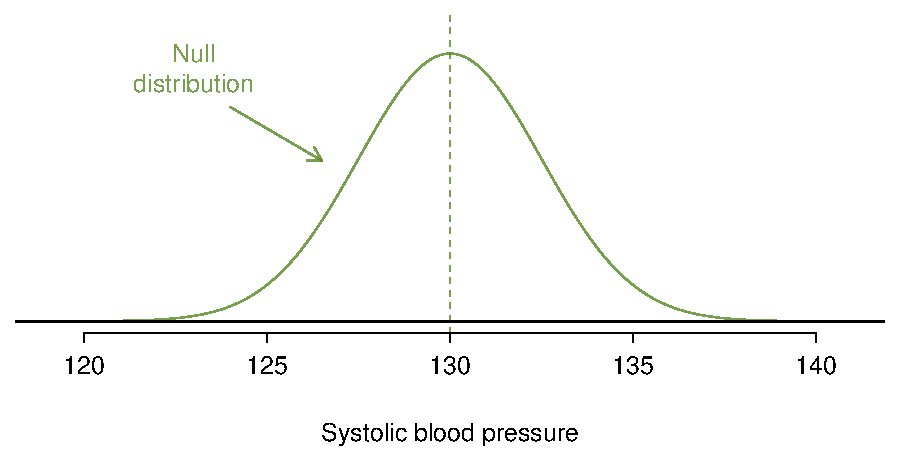
\includegraphics[width=0.9\textwidth]{4-6_samp_size_power/figures/power/power1.pdf}}
\only<2|handout:2>{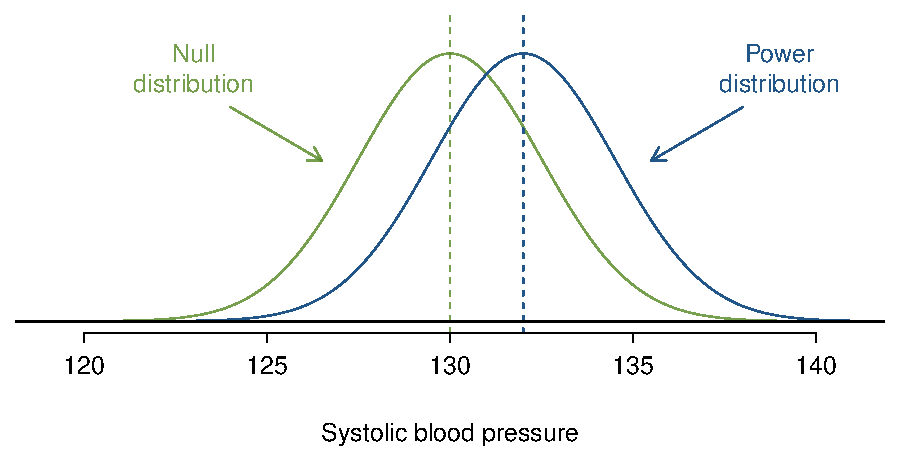
\includegraphics[width=0.9\textwidth]{4-6_samp_size_power/figures/power/power2.pdf}}
\only<3|handout:3>{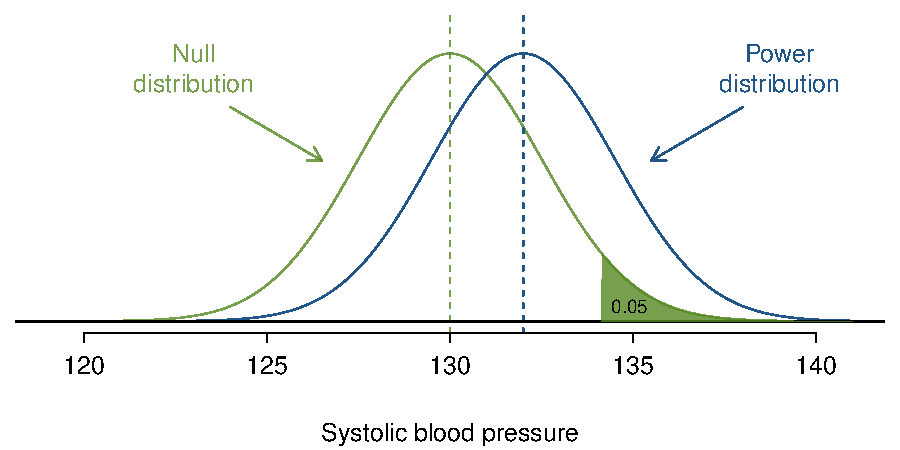
\includegraphics[width=0.9\textwidth]{4-6_samp_size_power/figures/power/power3.pdf}}
\only<4|handout:4>{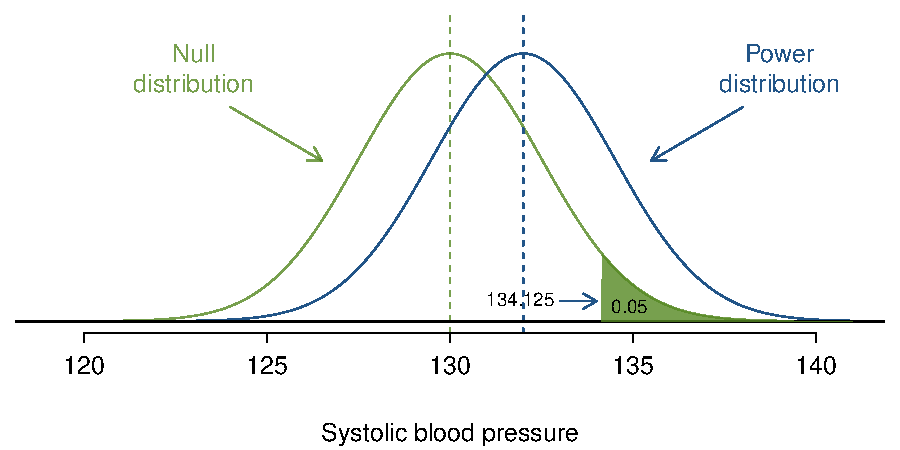
\includegraphics[width=0.9\textwidth]{4-6_samp_size_power/figures/power/power4.pdf}}
\only<5|handout:5>{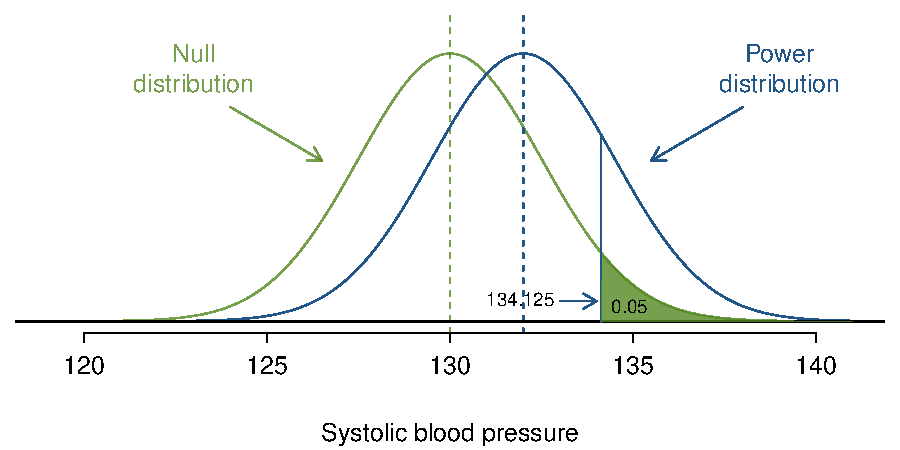
\includegraphics[width=0.9\textwidth]{4-6_samp_size_power/figures/power/power5.pdf}}
\only<6|handout:6>{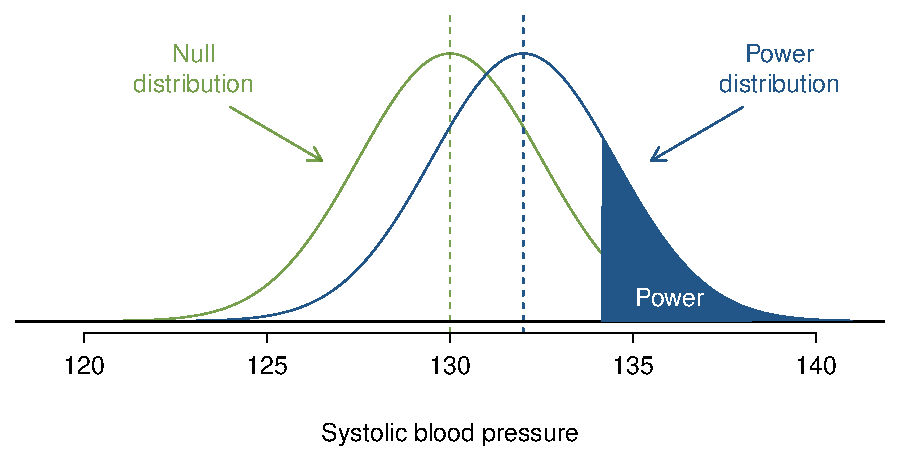
\includegraphics[width=0.9\textwidth]{4-6_samp_size_power/figures/power/power6.pdf}}
\end{center}


\end{frame}

%%%%%%%%%%%%%%%%%%%%%%%%%%%%%%%%%%%%

\begin{frame}
\frametitle{Achieving desired power}

There are several ways to increase power (and hence decrease type 2 error rate):

\pause

\begin{enumerate}

\item Increase the sample size.

\pause

\item Decrease the standard deviation of the sample, which essentially has the same effect as increasing the sample size (it will decrease the standard error). With a smaller $s$ we have a better chance of distinguishing the null value from the observed point estimate. This is difficult to ensure but cautious measurement process and limiting the population so that it is more homogenous may help.

\pause

\item Increase $\alpha$, which will make it more likely to reject $H_0$ (but note that this has the side effect of increasing the Type 1 error rate).

\pause

\item Consider a larger effect size. If the true mean of the population is in the alternative hypothesis but close to the null value, it will be harder to detect a difference.

\end{enumerate}

\end{frame}

%%%%%%%%%%%%%%%%%%%%%%%%%%%%%%%%%%%%

\begin{frame}
\frametitle{Recap - Calculating Power}

\begin{itemize}

\item Begin by picking a meaningful effect size $\delta$ and a significance level $\alpha$
\item Calculate the range of values for the point estimate beyond which you would reject $H_0$ at the chosen $\alpha$ level.
\item Calculate the probability of observing a value from preceding step if the sample was derived from a population where $\bar{x} \sim N(\mu_{H_0}+\delta,SE)$

\end{itemize}

\end{frame}


%%%%%%%%%%%%%%%%%%%%%%%%%%%%%%%%%%%%

\begin{frame}
\frametitle{Example - Using power to determine sample size}

{\footnotesize
Going back to the blood pressure example, how large a sample would you need if you wanted 90\% power to detect a 4 mmHg increase in average blood pressure for the hypothesis that the population average is greater than 130 mmHg at $\alpha = 0.05$? \\
\pause
\[ \hl{Given:~~} H_0: \mu = 130,~~H_A: \mu > 130,~~\alpha=0.05,~~\beta=0.10,~~\sigma=25,~~\delta=4 \]
~\\
\pause
\hl{Step 1:} Determine the cutoff -- in order to reject $H_0$ at $\alpha = 0.05$, we need a sample mean that will yield a Z score of at least 1.65.
\[\bar{x} > 130 + 1.65 \frac{25}{\sqrt{n}} \]
\pause
\hl{Step 2:} Set the probability of obtaining the above $\bar{x}$ if the true population is centered at 130 + 4 = 134 to the desired power, and solve for $n$.
\[P\left(\bar{x} > 130 + 1.65 \frac{25}{\sqrt{n}} \right) = 0.9\]
\[ P\left(Z > \frac{\left(130 + 1.65 \frac{25}{\sqrt{n}}\right) - 134}{\frac{25}{\sqrt{n}}} \right) = P\left(Z > 1.65 - 4\frac{\sqrt{n}}{25} \right) = 0.9 \]
}
\end{frame}

%%%%%%%%%%%%%%%%%%%%%%%%%%%%%%%%%%%%

\begin{frame}
\frametitle{Example - Using power to determine sample size (cont.)}

You can either directly solve for $n$, or use computation to calculate power for various $n$ and determine the sample size that yields the desired power:

\pause

\begin{center}
\only<2>{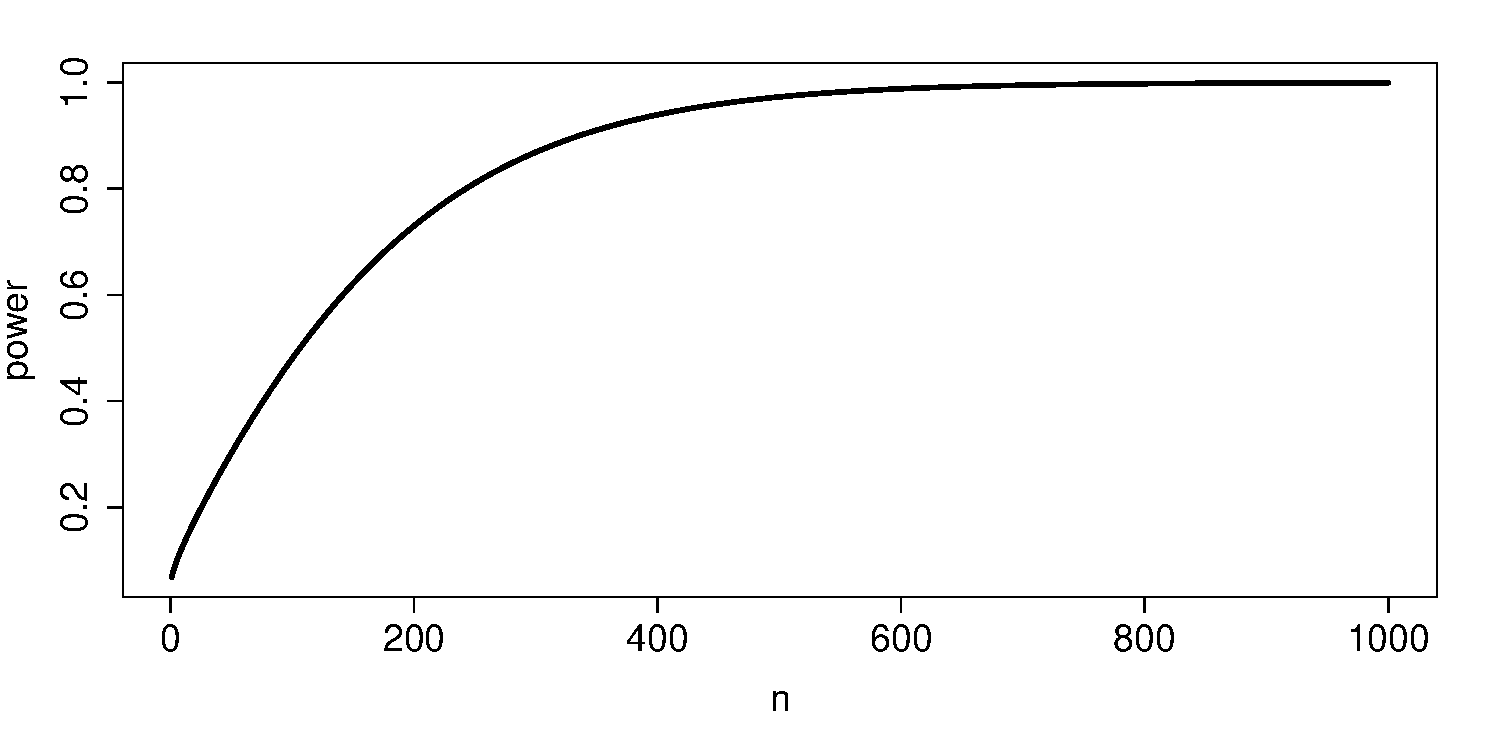
\includegraphics[width=0.8\textwidth]{4-6_samp_size_power/figures/power_curve/power_curve1.pdf}}
\only<3>{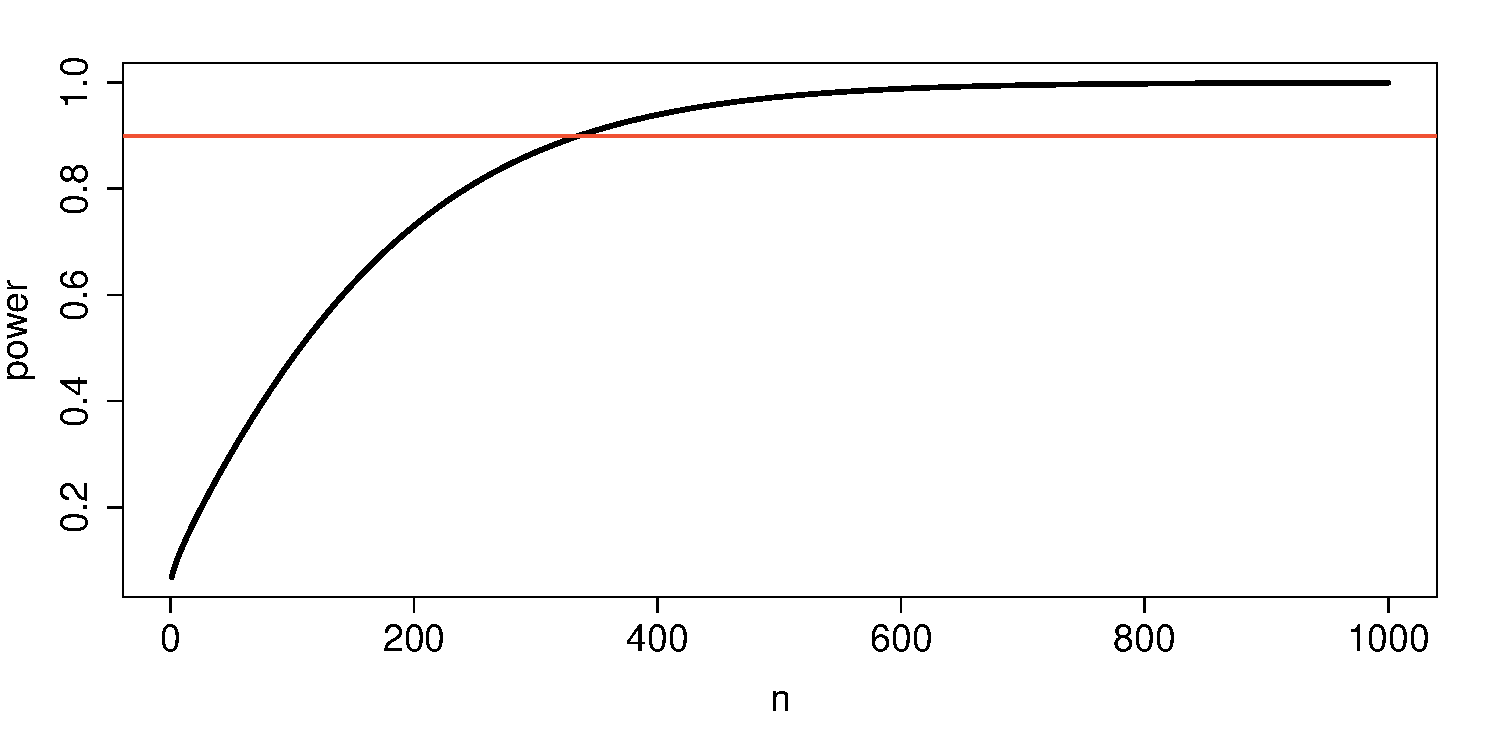
\includegraphics[width=0.8\textwidth]{4-6_samp_size_power/figures/power_curve/power_curve2.pdf}}
\only<4->{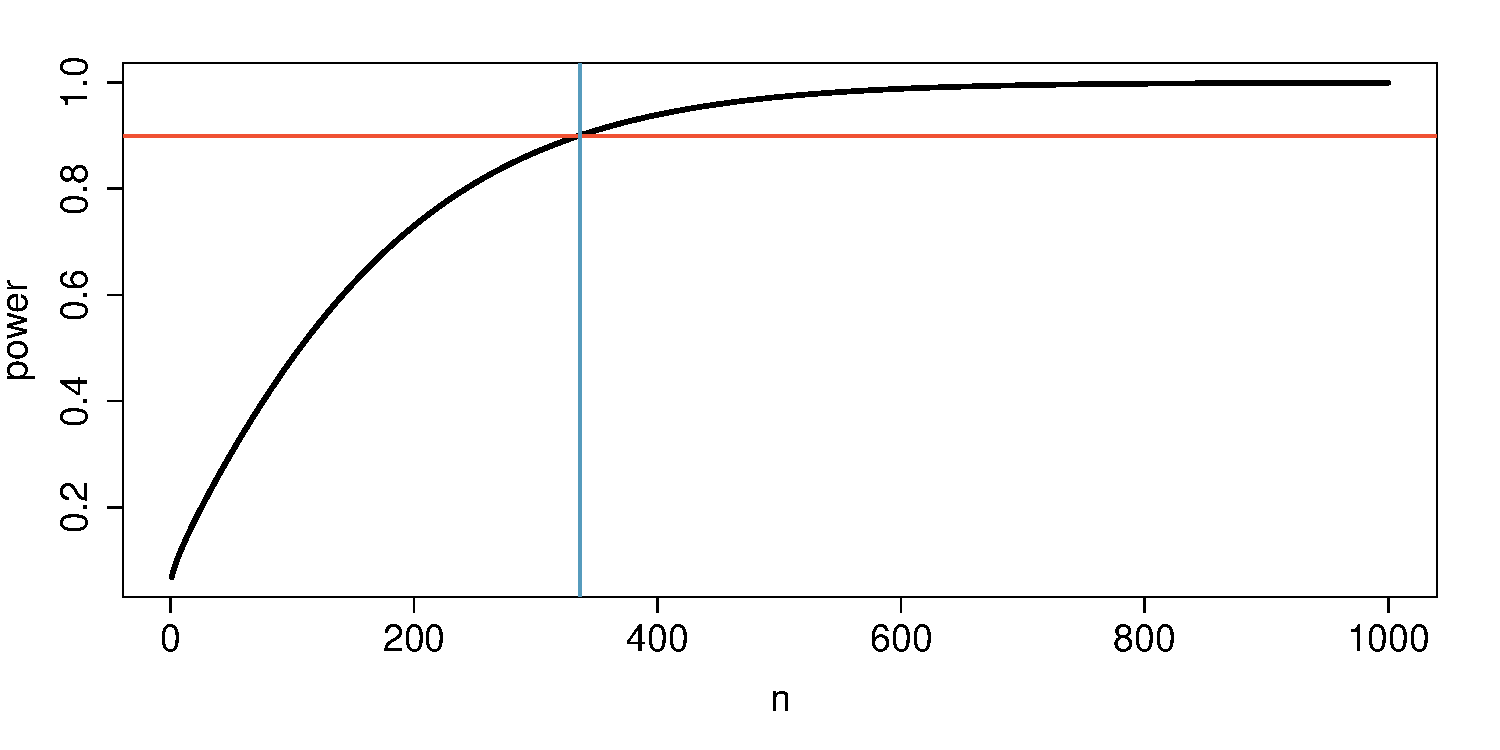
\includegraphics[width=0.8\textwidth]{4-6_samp_size_power/figures/power_curve/power_curve3.pdf}}
\end{center}

\vspace{-5mm}

\only<5->{
For $n=336$, $\text{power} = 0.9002$, therefore we need 336 subjects in our sample to achieve the desired level of power for the given circumstance.
}

\end{frame}

%%%%%%%%%%%%%%%%%%%%%%%%%%%%%%%%%%%%

\section{Statistical vs. practical significance}

%%%%%%%%%%%%%%%%%%%%%%%%%%%%%%%%%%%%

\begin{frame}
\frametitle{}

\pq{All else held equal, will the p-value be lower if $n = 100$ or $n = 10,000$?}

\begin{enumerate}[(a)]
\item $n = 100$
\solnMult{$n = 10,000$}
\end{enumerate}

\soln{\pause \pause
Suppose $\bar{x} = 50$, $s = 2$, $H_0: \mu = 49.5$, and $H_A: \mu \ge 49.5$.\\
\pause
\begin{eqnarray*}
Z_{n = 100} &=& \frac{50 - 49.5}{\frac{2}{\sqrt{100}}} \pause = \frac{50 - 49.5}{\frac{2}{10}} = \frac{0.5}{0.2} = 2.5,~~~\text{p-value} = 0.0062 \\
\pause
Z_{n = 10000} &=& \frac{50 - 49.5}{\frac{2}{\sqrt{10000}}} \pause = \frac{50 - 49.5}{\frac{2}{100}} = \frac{0.5}{0.02} = 25,~~~\text{p-value} \approx 0
\end{eqnarray*}
\pause
\begin{center}
As $n$ increases - $SE$ $\downarrow$, $Z$ $\uparrow$, p-value $\downarrow$
\end{center}
}

\end{frame}

%%%%%%%%%%%%%%%%%%%%%%%%%%%%%%%%%%%%

\begin{frame}

\dq{Test the hypothesis $H_0: \mu = 10$ vs. $H_A: \mu > 10$ for the following 8 samples. Assume $\sigma = 2$.}

\begin{center}
\renewcommand\arraystretch{1.5}
\begin{tabular}{l | c | c | c | c}
\hline
$\bar{x}$		& $10.05$ 	& $10.1$ 		& $10.2$  		 \\ 
\hline
\hline
\red{$n = 30$}  
	& \soln{\only<1>{\textcolor{white}{$p-value = 0.45$}}		\only<2->{$p-value = 0.45$}}	
	& \soln{\only<1-3>{\textcolor{white}{$p-value = 0.39$}}		\only<4->{$p-value = 0.39$}} 		
	& \soln{\only<1-5>{\textcolor{white}{$p-value = 0.29$}}		\only<6->{$p-value = 0.29$}} \\
\hline
\hline
\red{$n = 5000$} 
	& \soln{\only<1-2>{\textcolor{white}{$p-value = 0.39$}}		\only<3->{$p-value = 0.04$}}	
	& \soln{\only<1-4>{\textcolor{white}{$p-value = 0.0002$}}		\only<5->{$p-value = 0.0002$}}	
	& \soln{\only<1-6>{\textcolor{white}{$p-value \approx 0$}}	\only<7->{$p-value \approx 0$}}	 \\
\hline
\end{tabular}
\end{center}

\pause

\soln{\only<8->{When $n$ is large, even small deviations from the null (small effect sizes), which may be considered practically insignificant, can yield statistically significant results.}}

\end{frame}

%%%%%%%%%%%%%%%%%%%%%%%%%%%%%%%%%%%%

\begin{frame}
\frametitle{Statistical vs. practical significance}

\begin{itemize}

\item Real differences between the point estimate and null value are easier to detect with larger samples.

\item However, very large samples will result in statistical significance even for tiny differences between the sample mean and the null value (\hl{effect size}), even when the difference is not practically significant.

\item This is especially important to research: if we conduct a study, we want to focus on finding meaningful results (we want observed differences to be real, but also large enough to matter).

\item The role of a statistician is not just in the analysis of data, but also in planning and design of a study.
\end{itemize}

\begin{center}{\footnotesize
\textit{``To call in the statistician after the experiment is done may be no more than asking him to perform a post-mortem examination: he may be able to say what the experiment died of.''} -- R.A. Fisher
}\end{center}

\end{frame}

%%%%%%%%%%%%%%%%%%%%%%%%%%%%%%%%%%%%